\documentclass[9pt,fleqn,twoside,twocolumn]{stdglobal}

\fancypagestyle{titlepagestyle}{
  \fancyhf{}
  \fancyhead[L]{\footnotesize\itshape Seminar (Illustrative Visualization) 2021/2022}
  % \fancyfoot[C]{\footnotesize\bigskip\thepage/\pageref{LastPage}}
  % \fancyfoot{}
  \fancyfoot[C]{\footnotesize\bigskip\thepage}
  \fancyfoot[RO]{\footnotesize\bigskip\copyright\ Markus Pawellek, \today}
  \renewcommand{\footrulewidth}{0.5pt}
  \renewcommand{\headrulewidth}{0pt}
}

\fancypagestyle{mystyle}{
  \fancyhf{}
  \fancyfoot[C]{\footnotesize\bigskip\thepage}
  \fancyfoot[RO]{\footnotesize\bigskip\copyright\ Markus Pawellek, \today}
  % \fancyhead[LO,RE]{\footnotesize \thetitle} %left
  % \fancyhead[RO,LE]{\footnotesize \theauthor} %right
  % \fancyhead[LO,RE]{\footnotesize \ \smallskip}
  \fancyhead[LE]{\footnotesize\itshape Photic Extremum Lines \smallskip} %right
  \fancyhead[RO]{\footnotesize\itshape Seminar (Illustrative Visualization) 2021/2022\smallskip } %right
  \renewcommand{\headrulewidth}{0.5pt}
  \renewcommand{\footrulewidth}{0.5pt}
}

\usepackage{titlesec}
\titleformat{\section}{\normalfont\bfseries}{\thesection}{1em}{}

\title{Photic Extremum Lines}
\author{Markus Pawellek}
\date{\today}

\hypersetup{
  pdftex,
  % pdfauthor={Your Name},
  % pdftitle={The Title},
  % pdfsubject={\@title},
  pdfkeywords={Non-Photorealistic Rendering; Feature Lines; View-Dependent Object-Space Algorithm; Contours; Silhouettes; Suggestive Contours; Photic Extremum Lines; Illumination},
  % pdfproducer={Latex with hyperref},
  % pdfcreator={pdflatex, or other tool}
}

\bibliography{references}

\pagestyle{mystyle}

\begin{document}

\selectlanguage{english}

\thispagestyle{titlepagestyle}

\twocolumn[{\begin{@twocolumnfalse}%
  \begin{center}
    \Large
    \bfseries
    Photic Extremum Lines
  \end{center}%
  %\hfill\rule{0.5\textwidth}{0.5pt}\hfill
  \vspace{1pt}
  \begin{center}
    Markus Pawellek \\
    markus.pawellek@mailbox.org
  \end{center}
  \vspace{1em}
  \begin{center}
    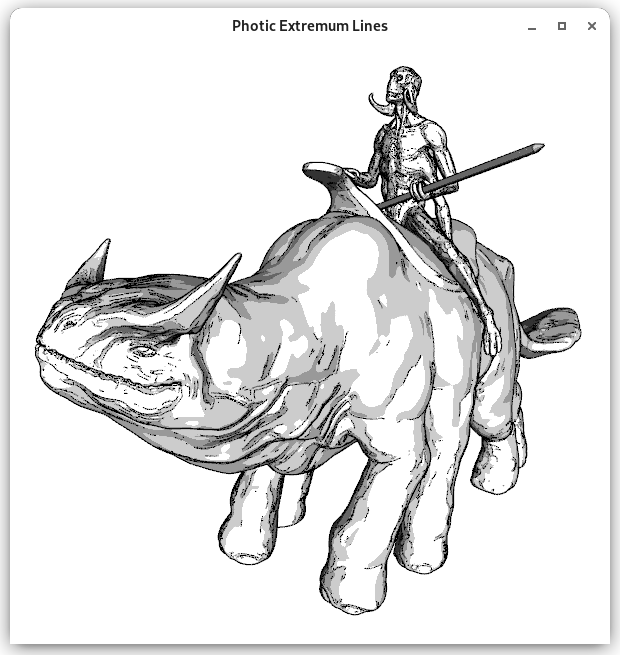
\includegraphics[width=0.24\textwidth,trim={15px 15 15 50},clip]{images/rider.png}
    \hfill
    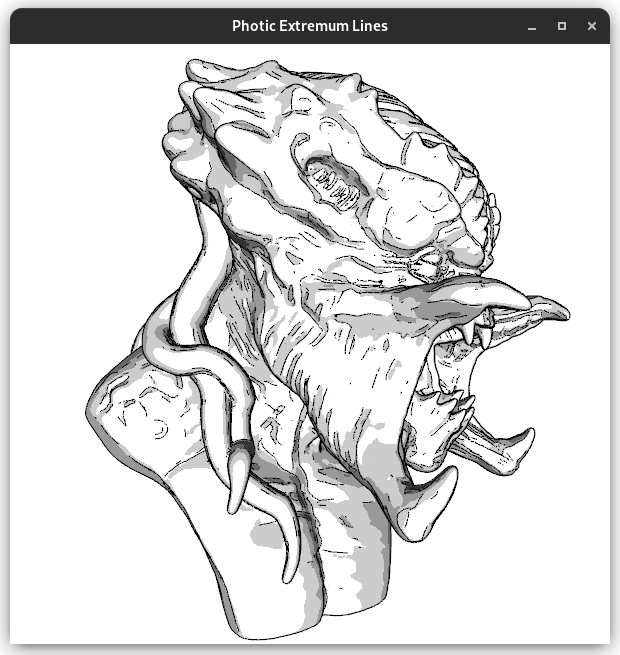
\includegraphics[width=0.24\textwidth,trim={15px 15 15 50},clip]{images/predator-intro.png}
    \hfill
    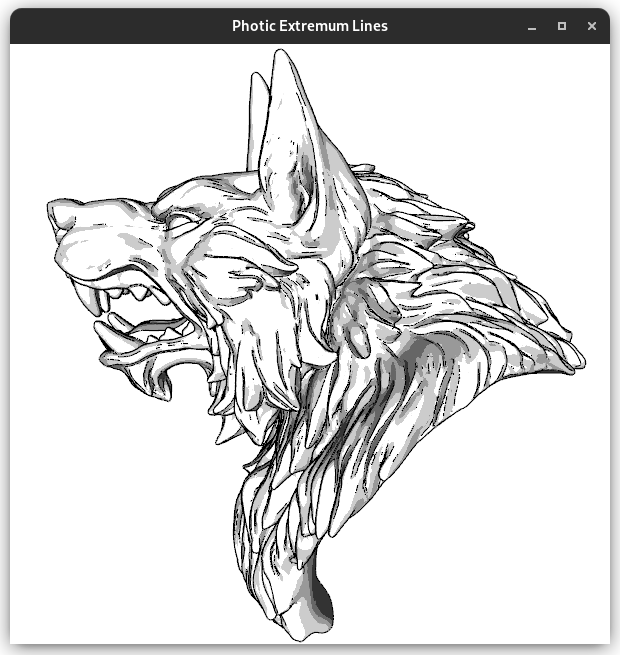
\includegraphics[width=0.24\textwidth,trim={15px 15 15 50},clip]{images/werewolf-intro.png}
    \hfill
    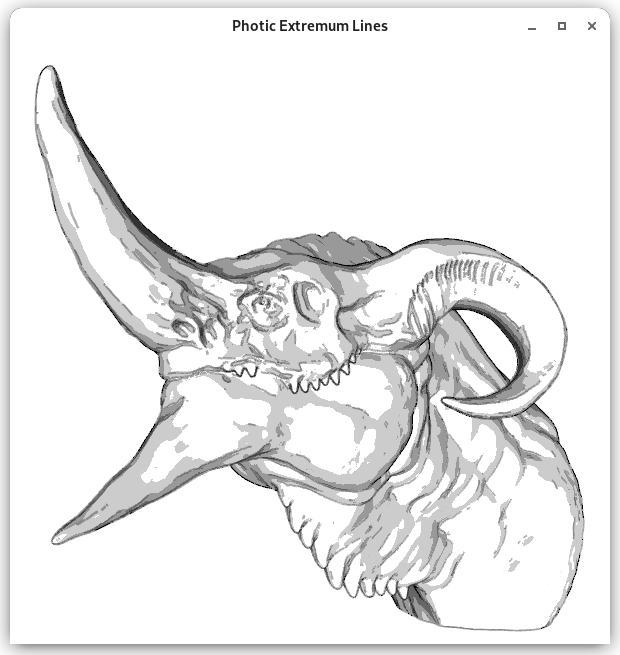
\includegraphics[width=0.24\textwidth,trim={15px 15 15 50},clip]{images/dragon-head-contour-pel-toon-shader.png}
  \end{center}
  \vspace{2em}
  \hrule
  \begin{abstract}
    \itshape
    \noindent
    In the field of illustrative visualization, feature lines are essential for conveying the shape of a given object.
    Photic extremum lines (PELs) are a type of feature line which are, besides normal and view position, dependent on the illumination.
    quis nostrud exercitation ullamco laboris nisi ut aliquip ex ea commodo
    consequat. Duis aute irure dolor in reprehenderit in voluptate velit esse
    cillum dolore eu fugiat nulla pariatur. Excepteur sint occaecat cupidatat non
    proident, sunt in culpa qui officia deserunt mollit anim id est laborum.
    \\

    \noindent
    \textbf{Keywords:}
    \parbox[t]{0.8\textwidth}{Non-Photorealistic Rendering, Feature Lines, View-Dependent Object-Space Algorithm, Contours, Silhouettes, Suggestive Contours, Photic Extremum Lines, Illumination}
  \end{abstract}
  \hrule
  \vspace{3em}
\end{@twocolumnfalse}}]

\begin{figure*}
    \centering
    \begin{subfigure}[b]{0.24\textwidth}
      \centering
      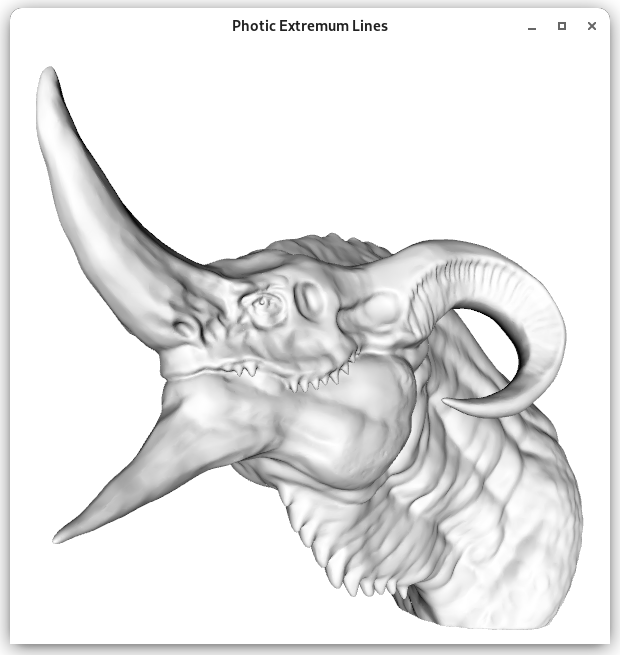
\includegraphics[width=0.95\textwidth,trim={15px 15 15 50},clip]{images/dragon-head-vertex-lighting.png}
      \caption{Illumination}
    \end{subfigure}%
    \hfill%
    \begin{subfigure}[b]{0.24\textwidth}
      \centering
      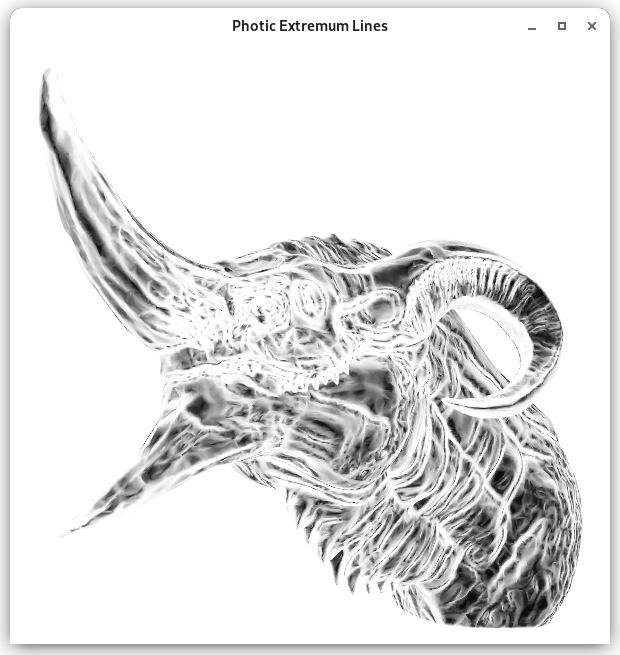
\includegraphics[width=0.95\textwidth,trim={15px 15 15 50},clip]{images/dragon-head-light-variation.png}
      \caption{Variation}
    \end{subfigure}%
    \hfill%
    \begin{subfigure}[b]{0.24\textwidth}
      \centering
      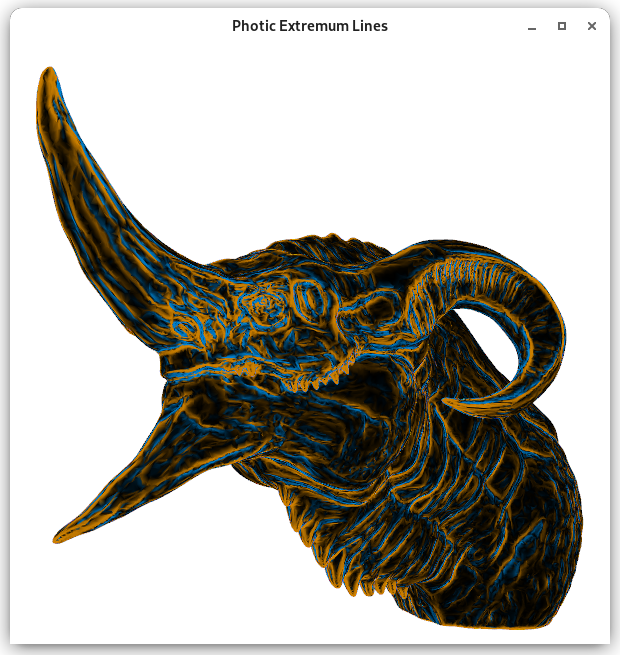
\includegraphics[width=0.95\textwidth,trim={15px 15 15 50},clip]{images/dragon-head-light-variation-slope.png}
      \caption{Variation Slope}
    \end{subfigure}%
    \hfill
    \begin{subfigure}[b]{0.24\textwidth}
      \centering
      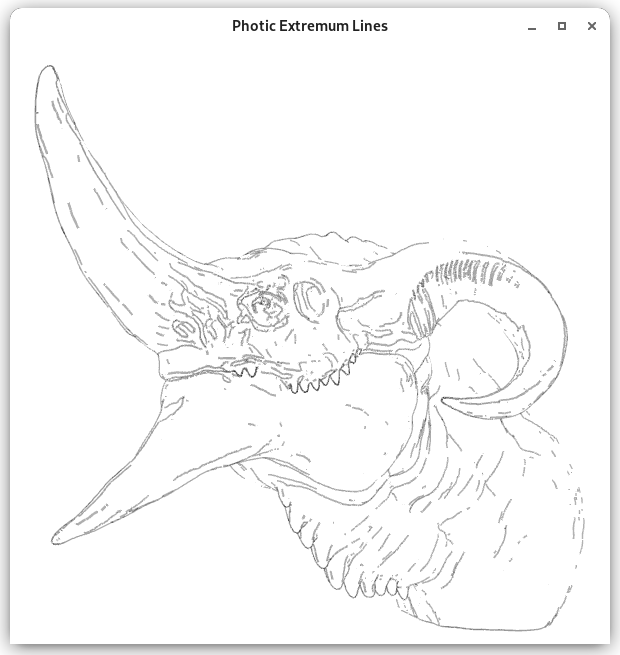
\includegraphics[width=0.95\textwidth,trim={15px 15 15 50},clip]{images/dragon-head-pel-shader.png}
      \caption{PELs}
    \end{subfigure}%
    \caption{\textbf{Short Summary Part}\\
    Lorem ipsum dolor sit amet, consectetur adipisicing elit, sed do eiusmod
    tempor incididunt ut labore et dolore magna aliqua. Ut enim ad minim veniam,
    quis nostrud exercitation ullamco laboris nisi ut aliquip ex ea commodo
    consequat. Duis aute irure dolor in reprehenderit in voluptate velit esse
    cillum dolore eu fugiat nulla pariatur. Excepteur sint occaecat cupidatat non
    proident, sunt in culpa qui officia deserunt mollit anim id est laborum.}
  \end{figure*}

\section{Introduction}
  Illustrative visualization is the science and art of effectively communicating known aspects of scientific data in an accurate and intuitive way.
  Especially for the rendering of volumetric data sets in medicine, it is a valuable tool to reduce a vast amount of complex information to its essence.
  In this respect, photorealistic rendering techniques are suboptimal because they are not able to efficiently depict features of interest.
  Our knowledge of human cognition shows that, artistic drawings or paintings, in comparison to a photograph of the same scene, seem to be more suitable for communication and more pleasing in visual experience \autocite{xie2007}.
  Therefore non-photorealistic rendering techniques, typically inspired by artistic styles, are used to create such illustrations.
  \autocite{viola2005}%
  \footnote{In this report, citations concerning more than one sentence are given at the end of the respective paragraph.}

  Feature lines represent a given data set as a line drawing to mimic hand-drawn illustrations.
  In such a way, a large amount of information can be communicated in a succinct manner by taking advantage of human visual acuity.
  Used as an abstraction tool in illustrative visualization, feature lines convey the shape of objects much more efficiently compared to a photograph.
  \autocite{xie2007,isenberg2003,viola2005}

  There are many different types of commonly-used feature lines, such as contours \autocite{isenberg2003}, suggestive contours \autocite{decarlo2003}, ridge-valley lines \autocite{ohtake2004}, apparent ridges \autocite{judd2007}, and demarcating curves \autocite{kolomenkin2008}.
  Typically, these only depend on the surface geometry, such as normal and curvature, and possibly the view position.
  However, human perception is highly sensitive to high variations in illumination.
  As a consequence, for conveying the shape of objects according to human perception, feature lines should also depend on the lighting of an object.
  \autocite{xie2007,zhang2011}

  In this report, we present the concept and implementation of photic extremum lines (PELs), one of the first types of feature lines exhibiting a dependency on illumination.
  PELs have been first introduced in \textcite{xie2007} and further developed in \textcite{zhang2010}.
  Strongly inspired by the edge detection techniques for 2D images, they are characterized by a sudden change of illumination on the surface of a 3D object.
  Since their computation is taken out in object space, PELs are flexible and enable further post-processing such as line stylization and shading \autocite{isenberg2003}.
  Furthermore, by manipulating the illumination of an object, the user can take full control to adjust the rendering output and achieve desired illustration results.
  Implementations for PELs can be done for the CPU and GPU, nowadays, achieving real-time performance.
  \autocite{xie2007,zhang2010}

\section{Related Work}
  The main references of this report are

\section{Mathematical Preliminaries}
  \begin{definition}[Mesh Function]
    \[
      \function{f}{S}{\setReal}
    \]
  \end{definition}

  \begin{definition}[(First Fundamental Form Triangle)]
    \[
      \mathrm{I}_{uv} \define
      \begin{pmatrix}
        \norm{u}^2 & \scalarProduct{u}{v} \\
        \scalarProduct{u}{v} & \norm{v}^2
      \end{pmatrix}
    \]
    \[
      \mathrm{I}^{-1}_{uv} = \frac{\adj \mathrm{I}_{uv}}{\det \mathrm{I}_{uv}} =
      \frac{1}{\norm{u}^2\norm{v}^2 - \absolute{\scalarProduct{u}{v}}}
      \begin{pmatrix}
        \norm{v}^2 & -\scalarProduct{u}{v} \\
        -\scalarProduct{u}{v} & \norm{u}^2
      \end{pmatrix}
    \]
  \end{definition}

  \begin{definition}[(Gradient Triangle)]
    \[
      [\nabla f]_{uv} = \mathrm{I}^{-1}_{uv}
      \begin{pmatrix}
        \Delta_u f \\
        \Delta_v f
      \end{pmatrix}
    \]
    \[
      \nabla f =
      \begin{pmatrix}
        u & v
      \end{pmatrix}
      [\nabla f]_{uv}
    \]
  \end{definition}

  \begin{definition}
    \[
      \partial_w f(x) \define \scalarProduct{\nabla f(x)}{w}
    \]
    \[
      \mathscr{D}_f g(x) \define \scalarProduct{\nabla g(x)}{\frac{\nabla f(x)}{\norm{\nabla f(x)}}}
    \]
  \end{definition}

  \begin{figure}
    \centering
    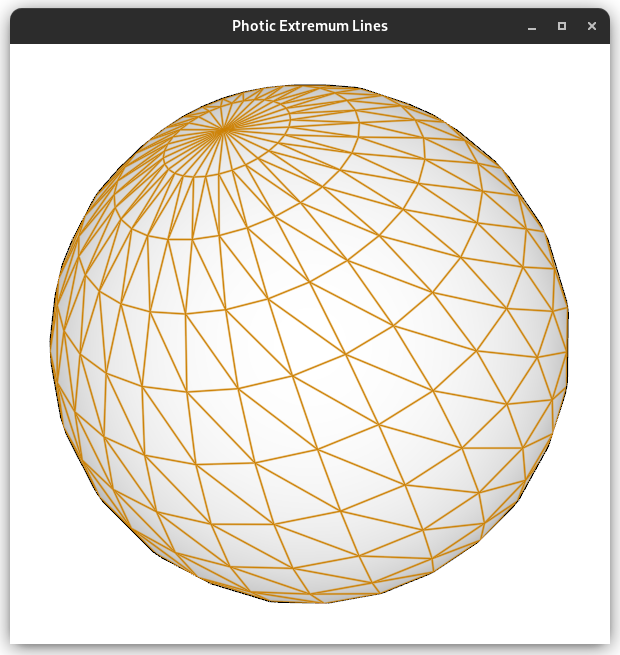
\includegraphics[width=0.6\linewidth,trim={15px 15 15 50},clip]{images/sphere-wireframe.png}
    \caption{Triangulated Meshes}
  \end{figure}

\section{Photic Extremum Lines}
  \begin{definition}[(Photic Extremum Lines)]
    Let $S$ be a smooth surface patch and $\function{φ}{S}{\setReal}$ three-times continuously differentiable scalar illumination function.
    The set of photic extremums over $S$ with respect to $φ$ consists of all points $x\in S$ where the variation of illumination in the direction of its gradient reaches a local maximum.
    In other words, such that the following holds.
    \[
      \mathscr{D}_φ\norm{\nabla φ}(x) = 0
      \separate
      \mathscr{D}^2_φ\norm{\nabla φ}(x) < 0
    \]
  \end{definition}

\section{Algorithm}

  \begin{tcolorbox}[%
    colframe=black,
    colbacktitle=white,
    coltitle=black,
    colback=mathdefback,
    attach boxed title to top center={yshift=-2mm},
    enhanced,
    titlerule=0.1pt,
    boxrule=0.5pt,
    arc=5pt,
    breakable,
    width=\linewidth,
    title=Algorithm
  ]
    Lorem ipsum dolor sit amet, consectetur adipisicing elit, sed do eiusmod
    tempor incididunt ut labore et dolore magna aliqua. Ut enim ad minim veniam,
    quis nostrud exercitation ullamco laboris nisi ut aliquip ex ea commodo
    consequat. Duis aute irure dolor in reprehenderit in voluptate velit esse
    cillum dolore eu fugiat nulla pariatur. Excepteur sint occaecat cupidatat non
    proident, sunt in culpa qui officia deserunt mollit anim id est laborum.
  \end{tcolorbox}

  \begin{figure}
    \centering
    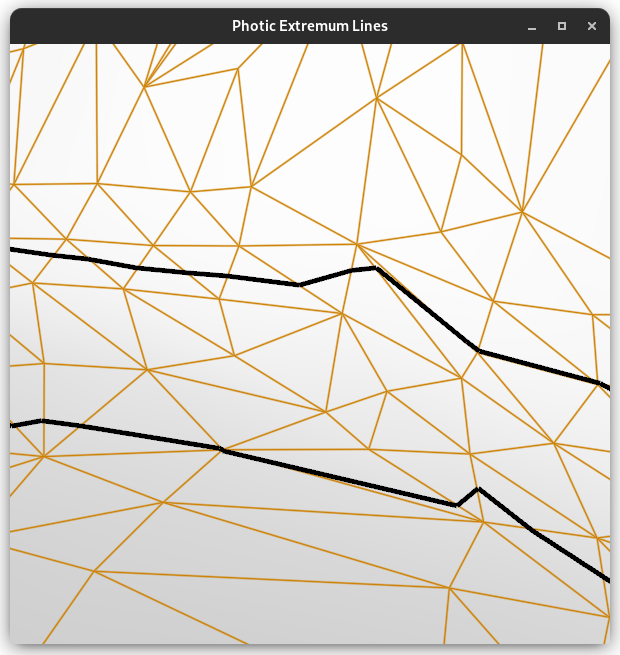
\includegraphics[width=\linewidth,trim={15px 15 15 50},clip]{images/subpolygon-lines.png}
    \caption{Sub-Polygon Feature Lines}
  \end{figure}

\section{Implementation}

\section{Results and Comparison}

  \begin{figure*}
      \centering
      \begin{subfigure}[b]{0.24\textwidth}
        \centering
        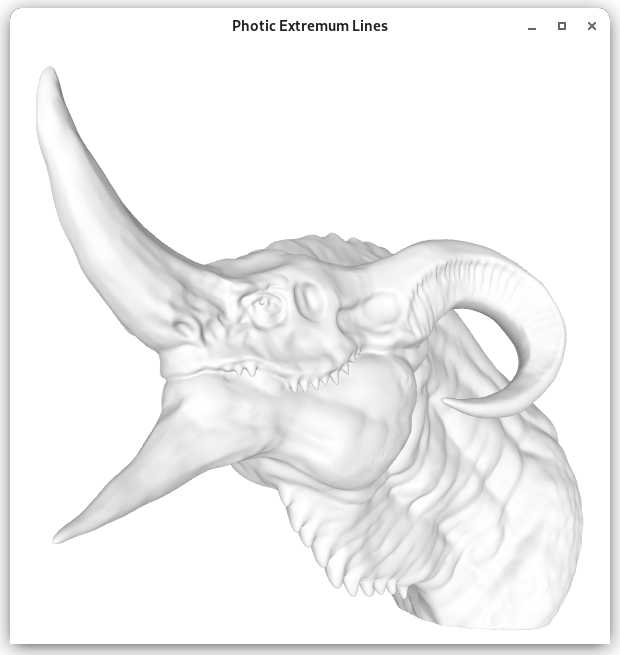
\includegraphics[width=0.95\textwidth,trim={15px 15 15 50},clip]{images/dragon-head-viewer-shader.png}
        \caption{Illumination}
      \end{subfigure}%
      \hfill%
      \begin{subfigure}[b]{0.24\textwidth}
        \centering
        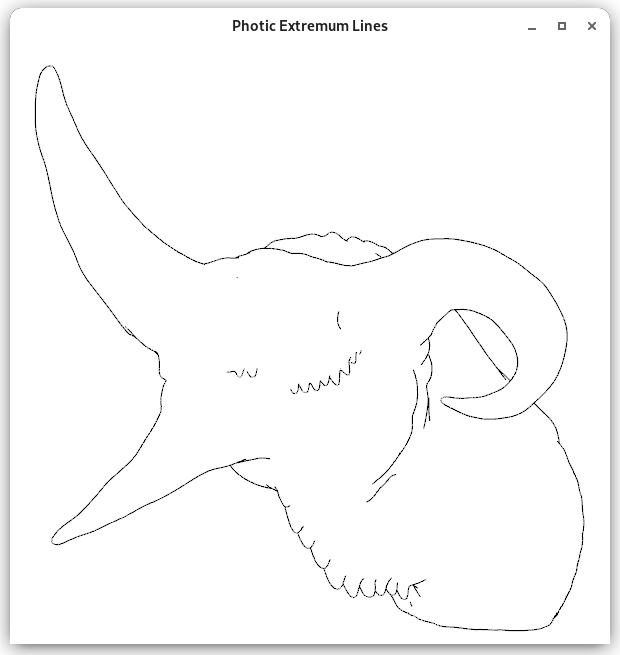
\includegraphics[width=0.95\textwidth,trim={15px 15 15 50},clip]{images/dragon-head-contours.png}
        \caption{Contours}
      \end{subfigure}%
      \hfill%
      \begin{subfigure}[b]{0.24\textwidth}
        \centering
        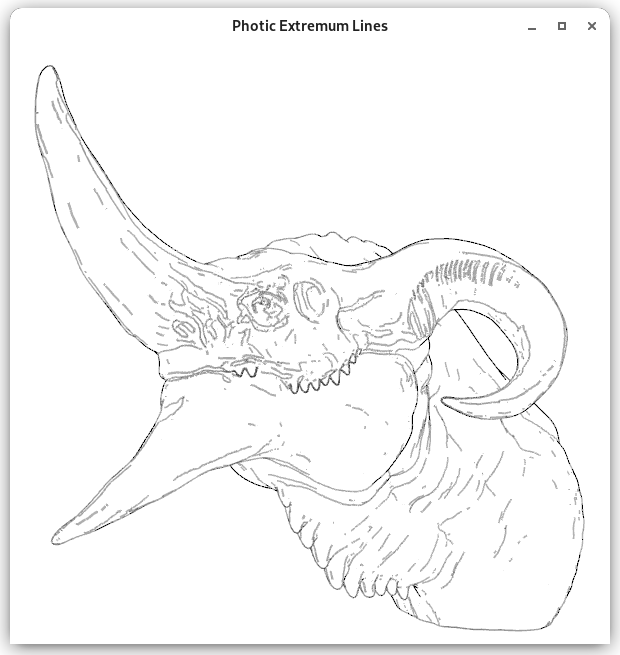
\includegraphics[width=0.95\textwidth,trim={15px 15 15 50},clip]{images/dragon-head-contour-pel-shader.png}
        \caption{Contours and PELs}
      \end{subfigure}%
      \hfill
      \begin{subfigure}[b]{0.24\textwidth}
        \centering
        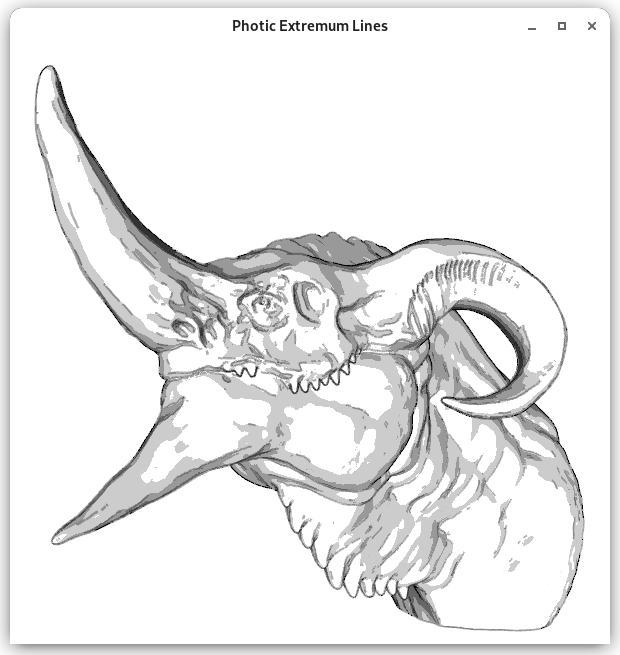
\includegraphics[width=0.95\textwidth,trim={15px 15 15 50},clip]{images/dragon-head-contour-pel-toon-shader.png}
        \caption{Contours, PELs, and Toon}
      \end{subfigure}%
      \caption{\textbf{Short Summary Part}\\
      Lorem ipsum dolor sit amet, consectetur adipisicing elit, sed do eiusmod
      tempor incididunt ut labore et dolore magna aliqua. Ut enim ad minim veniam,
      quis nostrud exercitation ullamco laboris nisi ut aliquip ex ea commodo
      consequat. Duis aute irure dolor in reprehenderit in voluptate velit esse
      cillum dolore eu fugiat nulla pariatur. Excepteur sint occaecat cupidatat non
      proident, sunt in culpa qui officia deserunt mollit anim id est laborum.}
    \end{figure*}

  \begin{figure}
    \centering
    \begin{subfigure}[b]{0.49\linewidth}
      \centering
      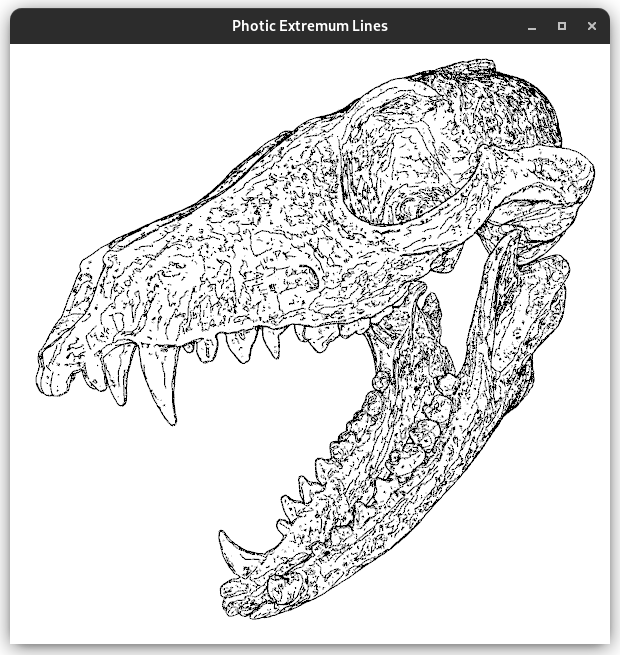
\includegraphics[width=\textwidth,trim={15px 15 15 50},clip]{images/fox-skull-threshold-low.png}
      \caption{Low}
    \end{subfigure}
    \begin{subfigure}[b]{0.49\linewidth}
      \centering
      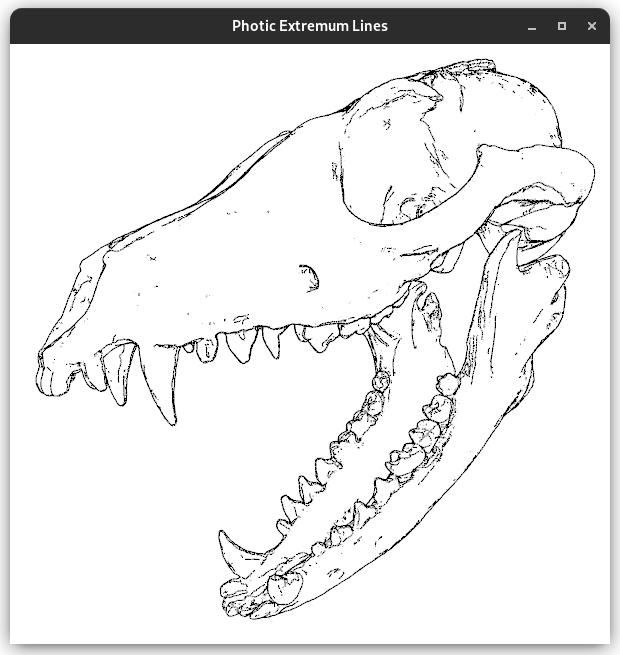
\includegraphics[width=\textwidth,trim={15px 15 15 50},clip]{images/fox-skull-threshold-mid.png}
      \caption{Mid}
    \end{subfigure}
    \caption{Effect of thresholding}
  \end{figure}

  \begin{figure}
    \centering
    \begin{subfigure}[b]{0.49\linewidth}
      \centering
      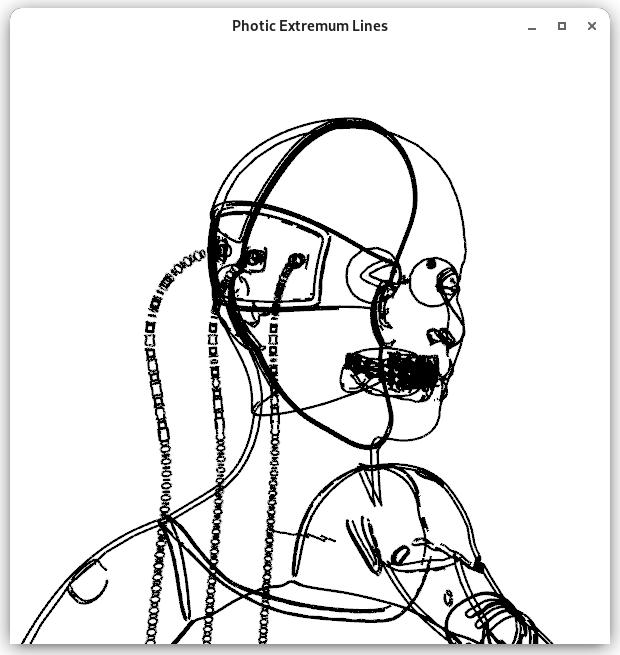
\includegraphics[width=\textwidth,trim={15px 15 15 50},clip]{images/cyborg-contour-pel-hidden-shader.png}
      \caption{Off}
    \end{subfigure}
    \begin{subfigure}[b]{0.49\linewidth}
      \centering
      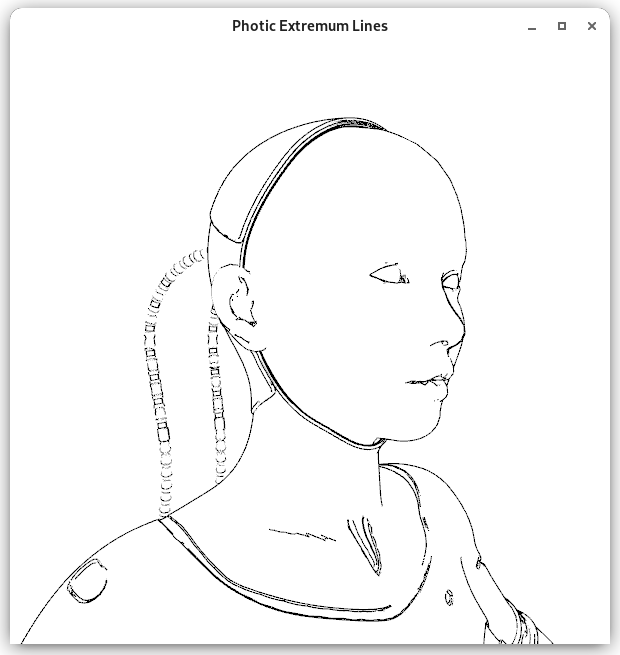
\includegraphics[width=\textwidth,trim={15px 15 15 50},clip]{images/cyborg-contour-pel-shader.png}
      \caption{On}
    \end{subfigure}
    \caption{Two-Pass Rendering for Hidden Line Removal}
  \end{figure}

  \begin{figure}
    \centering
    \begin{subfigure}[b]{\linewidth}
      \centering
      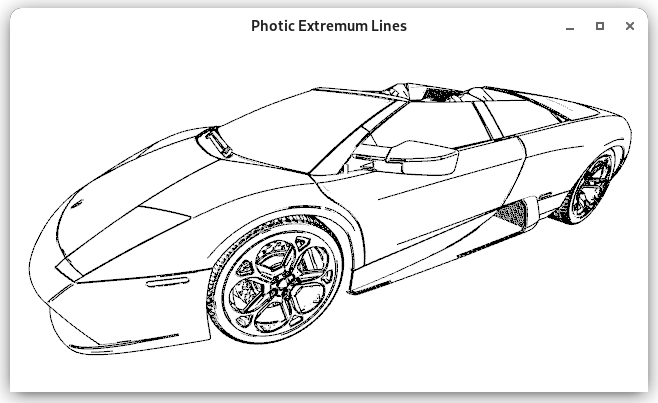
\includegraphics[width=\textwidth,trim={15px 15 15 50},clip]{images/lamborghini-front.png}
      \caption{Front}
    \end{subfigure}
    \begin{subfigure}[b]{\linewidth}
      \centering
      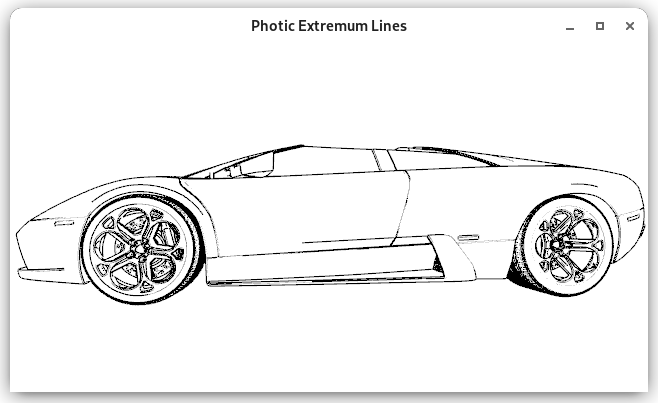
\includegraphics[width=\textwidth,trim={15px 15 15 50},clip]{images/lamborghini-side.png}
      \caption{Side}
    \end{subfigure}
    \caption{Nearly Perfect Line Extraction for Smooth Objects}
  \end{figure}

  \begin{figure}
    \centering
    \begin{subfigure}[b]{0.49\linewidth}
      \centering
      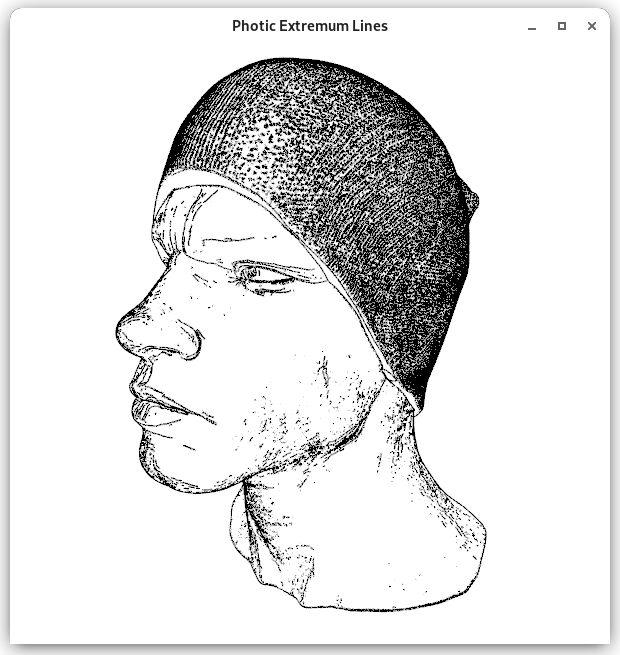
\includegraphics[width=\textwidth,trim={15px 15 15 50},clip]{images/head-contour-pel-shader.png}
      \caption{Contours and PELs}
    \end{subfigure}
    \begin{subfigure}[b]{0.49\linewidth}
      \centering
      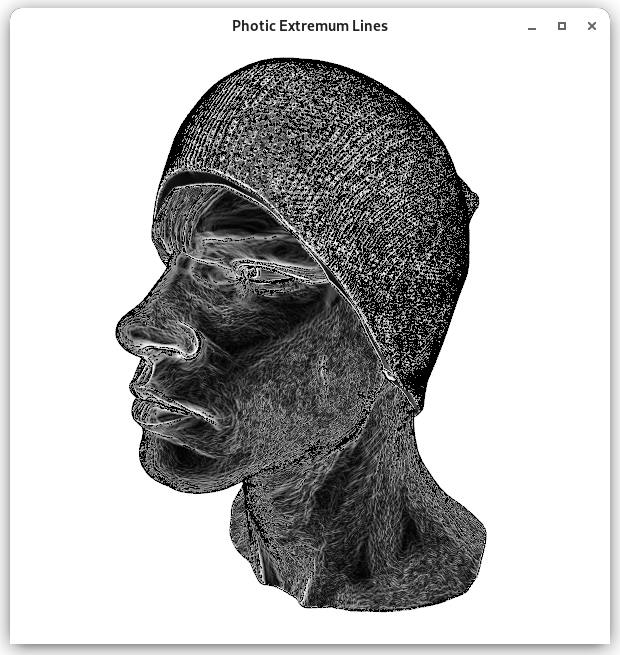
\includegraphics[width=\textwidth,trim={15px 15 15 50},clip]{images/head-light-variation.png}
      \caption{Variation}
    \end{subfigure}
    \caption{Erroneous Line Extraction for Noisy Objects}
  \end{figure}

\section{Conclusions}

\nocite{*}
\AtNextBibliography{\footnotesize}
\printbibliography[heading=bibintoc]

\appendix

\end{document}
